\chapter{Úvod}
Úlohou projektu bolo navrhnúť, implementovať a otestovať hybridnú chatovaciu P2P sieť obsahujúcu chatovacích peerov a registračné uzly. V~nasledujúcich kapitolách sú opísané dôležité časti projektu.

V~kapitole 2 prebieha úvodom do problematiky, ozrejmením relevantných pojmov. Kapitola 3 sa zaoberá komunikačným protokolom. V~kapitole 4 je opísaná jeho samotná implementácia. Kapitola 5 obsahuje informácie o~priebehu ladenia a testovania. Kapitola 6 poskytuje prehľad nad používaním programu. Posledná kapitola zhrňuje získané vedomosti a skúsenosti z~projektu.
 

\chapter{Súhrn pojmov}
Táto kapitola obsahuje prehľad a ozrejmenie základných pojmov súvisiacich s~problematikou tohto projektu. Informácie ohľadom P2P sietí boli čerpané hlavne z~prednášky v~predmete PDS \cite{p2p_fit} a súvisiaceho RFC dokumentu.

\section*{P2P sieť}

P2P sieť je možné definovať ako súbor nezávislých uzlov (označovaných ako \uv{peers}), ktoré sú prepojené a ich zdroje sú k~dispozícii iným uzlom v~tejto sieti. P2P siete sa nezaobídu bez funkčnej IP infraštruktúry a taktiež je nutné v~týchto sieťach riešiť problematiku adresovanie, smerovania, zabezpečenia a pod.
Základom každej P2P siete je logická sieť, ktorá je postavená nad existujúcou sieťovou infraštruktúrou. Logická sieť definuje spôsob prepojenia uzlov, smerovanie, vyhľadávanie informácie a pod. Medzi význačné vlastnosti P2P sietí patria: samorganizovateľnosť, autonómne chovanie, spoľahlivosť a životnosť uzlu. 
Všeobecne rozlišujeme dva typy P2P sietí: pravé, kde odobranie ľubovolného uzlu zo siete nemá vplyv na schopnosť poskytovať službu a hybridné, ktoré pre svoju činnosť využívajú centrálny uzol pre poskytovanie časti ponúkaných sieťových služieb (ako napr. autentizácia, indexovanie či inicializácia uzla). Na obrázku \ref{hybripp2p} \footnote{\url{https://www.slideshare.net/jamezsa/lecture-network-technologies-peertopeer-networks}} je zobrazená schéma hybridnej P2P siete. Viac informácií ohľadom P2P sietí je možné nájsť v~dokumente RFC 5694 \cite{rfc5694}.

\begin{figure}[H]
	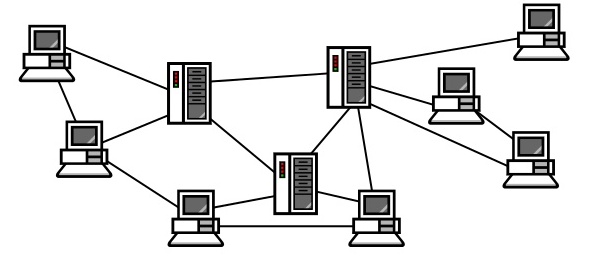
\includegraphics[width=\textwidth]{p2p_hybrid}
	\caption{Schéma hybridnej P2P siete}
	\label{hybripp2p}
\end{figure}

\section*{UDP}

UDP je základným protokolom transportnej vrstvy v~architektúre TCP/IP. Je tiež označovaný ako tzv. nespojovaný (\uv{connectionless}) protokol. Protokol prináša malé zaťaženie siete, no jeho nevýhodou je to, že sa neriešia prípady straty, poškodenia paketov, prípadne zmena poradia ich doručenia, a tiež môže dochádzať k~duplicite dát. Protokol UDP je podrobne opísaný v~RFC 768 \cite{rfc768}.


Na obrázku \ref{rpcmodel} je znázornený model RPC \footnote{\url{https://www.geeksforgeeks.org/operating-system-remote-procedure-call-rpc/}}. Klient odosiela požiadavku na server. Požiadavka sa na serveri vykoná a možná odpoveď sa posiela späť žiadateľovi, tj. klientovi. Server následne čaká na ďalších klientov a ich požiadavky.

\section*{Bencode}

Bencode je kódovanie používané peer-to-peer systémom na zdieľanie súborov \textit{BitTorrent} na ukladanie a prenos dát. Podporuje štyri rôzne typy hodnôt: reťazce, celé čísla, zoznamy a slovníky. Najčastejšie sa používa v~torrent súboroch, kde sú tieto metadátové súbory kódované slovníky práve pomocou Bencode. Viac podrobností ohľadom bencode a samotný algoritmus spôsob kódovania je možné nájsť na (neoficiálnej) Wiki stránke \footnote{\url{https://wiki.theory.org/index.php/BitTorrentSpecification\#Bencoding}}. Dokument obsahujúci špecifikáciu Bencode je BEP 3 \cite{bep3}.

\section*{JSON}

JSON (\uv{JavaScript Object Notation}) je spôsob zápisu dát (dátový formát) nezávislý na počítačovej platforme, určený pre prenos dát, ktoré môžu byť organizovaná v poliach alebo zoskupená v objektoch. Vstupom je ľubovoľná dátová štruktúra (číslo, reťazec, boolean, objekt alebo z nich zložené poľa), výstupom je vždy reťazec. Špecifikáciu JSON formátu je možné nájst v dokumente RFC 8259 \cite{rfc8259}.

\section*{RPC}

\uv{Remote Procedure Call} (RPC) je technika vzdialeného volania procedúr. Umožňuje programu vykonať kód na inom mieste, než je umiestnený volajúci program.

\begin{figure}[H]
	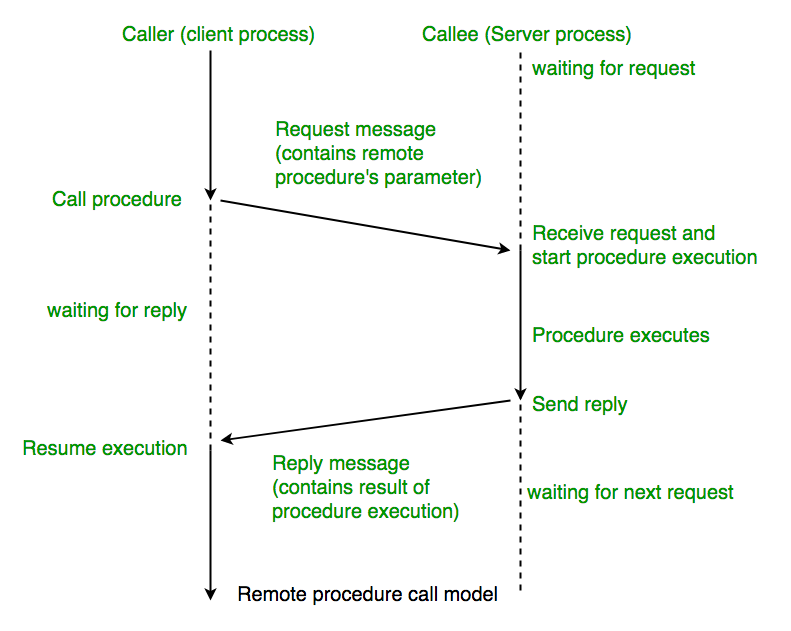
\includegraphics[width=\textwidth]{rpc}
	\caption{Model Remote Procedure Call}
	\label{rpcmodel}
\end{figure}


\chapter{Komunikačný protokol}

Peeri a registračné uzly používajú jednoduchý komunikačný protokol pozostávajúci z nižšie uvedených správ. Všetky správy medzi dvoma peerami, dvoma registračnými uzlami, či medzi peerom a registračným uzlom sú prenášané cez protokol UDP. Všetky správy majú JSON syntax, kde povinným atribútom je \textit{type}, ktorý špecifikuje typ správy. Pred prenosom cez UDP je obsah správy zakódovaný pomocou Bencode. Keďže protokol UDP negarantuje doručenie, tak sa na potvrdenie používa správa typu \texttt{ack}, ktorá v sebe nesie odkaz na jedinečný transakčný identifikátor správy, ktorú potvrdzuje. Ak dôjde pri spracovaní ľubovoľnej správy k chybe, príjemca správy posiela odosielateľovi správu typu \texttt{error}, ktorá okrem identifikátora transakcie obsahuje aj slovný popis problému, ku ktorému došlo. Správy typu \texttt{hello}, \texttt{update} a \texttt{error} nie je potrebné pomocou správy \texttt{ack} potvrdzovať. Na potvrdenie \texttt{ack} sa čaká maximálne 2 sekundy, potom najprv zresetovat stav spracovania súvisiaceho s nepotvrdenú správou a následne ohlásiť chybu na štandardný chybový výstup (program sa neukončí, iba upozorní používateľa o chybe). Všeobecne je možné správy mimo očakávaný stav protokolu zahadzovať. \\

\noindent Protokol podporuje nasledujúce správy:

\begin{verbatim}
HELLO := {"type":"hello", "txid":<ushort>, "username":"<string>", 
		  "ipv4":"<dotted_decimal_IP>", "port": <ushort>}   
		                      	
GETLIST := {"type":"getlist", "txid":<ushort>}     
                  	
LIST := {"type":"list", "txid":<ushort>, "peers": {<PEER_RECORD*>}}   
                    
PEER_RECORD := {"<ushort>":{"username":"<string>", 
		  "ipv4":"<dotted_decimal_IP>", "port": <ushort>}}     
		                    
MESSAGE := {"type":"message", "txid":<ushort>, "from":"<string>",
			"to":"<string>", "message":"<string>"}
			                      
UPDATE := {"type":"update", "txid":<ushort>, "db": {<DB_RECORD*>}}
                       
DB_RECORD := {"<dotted_decimal_IP>,<ushort_port>":{<PEER_RECORD*>}}
                       
DISCONNECT := {"type":"disconnect", "txid":<ushort>}
\end{verbatim}

\chapter{Popis implementácie}

Kapitola popisuje návrhové rozhodnutia, použité mechanizmy a zaujímavejšie časti implementácie. Programy sú napísané v~Pythone 3, vývoj prebiehal nad Pythonom 3.6 na Ubuntu 18.04 LTS.

\section{Chatovací peer}

Chatovací peer je implementovaný v~súbore \texttt{pds18-peer.py}. Peer po spracovaní argumentov vytvorí nové vlákno, ktoré obsluhuje príkazy z~RPC. V~tomto vlákne spustí TCP server na voľnom porte a informáciu o~IPv4 adrese a porte tohto servera uloží do súboru pre potreby RPC (viď podkapitola venujúca sa implementácii RPC). Medzi implementačne zaujímave príkazy patria \texttt{peers}, \texttt{message} a \texttt{reconnect}. 

V~prípade príkazu \texttt{peers} je nutné poslať správu \texttt{getlist} registračnému uzlu a čakať na odpoveď, ktorou je správa \texttt{list}. RPC vlákno spustí slučku, v~ktorej po každej desatine sekundy kontroluje, či sa príznak prijatia správy \texttt{list} nenastavil. Následne pošle \texttt{ack} registračnému uzlu na túto prijatú správu. Prijatú správu \texttt{list} pošle späť na RPC klienta, ktorý ju vypíše na svoj výstup. Každá prijatá správa \texttt{list} zároveň aktualizuje internú \uv{cache} mapovaní peerov, ktorú si každý peer udržiava. 

Táto cache sa využíva pri správe \texttt{message}, kde sa najskôr hľadajú informácie o~príjemcovi správy najskôr v~tejto cache. V~prípade, že sa záznam o~príjemcovi nenájde, pošle sa správa \texttt{getlist} pre získanie najaktuálnejšieho mapovania peerov. Ak sa ani v~tomto zozname nenájde záznam o~príjemcovi, chybové hlásenie o~tomto probléme sa vypíše na štandardný chybový výstup a proces odosielania správy končí. Ak záznam existuje, je správa odoslaná príjemcovi na IPv4 adresu a port z~nájdeného záznamu. V~prípade, že odosielateľ špecifikovaný v~RPC príkaze nesúhlasí s~menom peera, je vypísané chybové hlásenie a ďalej sa proces posielania správy pracuje s~menom odosielateľa uvedeného v~parametroch RPC príkazu \texttt{message}. 

Po prijatí príkazu \texttt{reconnect} z~RPC peer odošle správu \texttt{hello} svojmu registračnému uzlu s~nulovými položkami na mieste IPv4 adresy a portu, čím oznamuje registračnému uzlu, že sa odpája od neho. Následne posiela klasickú správu \texttt{hello} novému registračnému uzlu, ktorého IPv4 adresa a port sú definované v~parametroch RPC príkazu.

Po spustení RPC vlákna sa v~\uv{hlavnom} vlákne taktiež spúšťa periodický časovač, ktorý každých 10 sekúnd odosiela správu \texttt{hello} svojmu registračnému uzlu. Ďalej prichádza na rad časť spracovávania správ, ktoré môže peer prijať. Ak dôjde k~chybe pri benkódovaní, prípadne správa neobsahuje nutné položky, je vypísané chybové hlásenie s~popisom problému a odoslaná správa typu \texttt{error} odosielateľovi poškodenej správy, ktorá ako sekvenčné číslo použije číslo z~prijatej správy. V~prípade, že v~prijatej správe chýbalo sekvenčné číslo, alebo toto číslo bolo mimo rozsah typu \textit{unsigned short}, je v~správe typu \texttt{error} použité číslo 0 ako sekvenčné číslo. Po odoslaní správy od peera sa v~\uv{ACK} slovníku pre dané sekvenčné číslo nastaví hodnota False. 

Po prijatí potvrdenia sa hodnota pre sekvenčné číslo z~prijatého potvrdenia v~tomto slovníku zmení na True. Po uplynutí časovača nastaveného na dve sekundy sa znova skontroluje záznam v~slovníku \-- ak je stále False, potvrdenie nedorazilo a peer vypíše chybové hlásenie a pokračuje v~činnosti ďalej. Peer po prijatí správy \texttt{list} si aktualizuje svoju \uv{cache} mapovaní peerov a zmenou príznaku upozorní potenciálne čakajúce RPC vlákno na prijatie správy typu \texttt{list}. Po prijatí správ \texttt{message} a \texttt{list} peer odosiela potvrdenie o~doručení registračnému uzlu.

Po ukončení peera pomocou Ctrl-C (SIGINT) sa peer odpojí od svojho registračného uzla tak, že zašle správu \texttt{hello} s~nulovými položkami na mieste IPv4 adresy a portu. Taktiež vypína aktuálne bežiace časovače a uzatvára sockety.

Rôzne premenné je nutné používať vo vláknach aj časovačoch. Z~tohto dôvodu sú v~implementácii na globálnej úrovni a pre jednoduchšiu orientáciu medzi premennými vo funkciách ich názov obsahuje prefix \uv{g\_}.


\section{Registračný uzol}

V~implementácii registračného uzla (\texttt{pds18-node.py}) sa používajú rovnaké návrhové rozhodnutia a princípy ako u~peera, a preto je pre čitateľa odporúčané sa najskôr oboznámiť s~predchádzajúcou podkapitolou. Špecificky však registračný uzol pridáva periodické časovače, ktoré posielajú správy \texttt{message} susedom registračného uzla. Taktiež pridáva aj časovače na detekciu odpojenia svojho peera či suseda zo siete. 

Po detegovaní odpojenia si registračný uzol upravuje svoje interné zoznamy a slovník (databáza). Registračný uzol po prijatí správy \texttt{getlist} overuje, čí žiadajúci peer patrí medzi peerov daného uzla \-- ak nie, je odoslané chybové hlásenie peerovi, ktorý ho na svoj výstup vypíše. Pri úspechu kontroly je odoslaná správa typu \texttt{list}, ktorá obsahuje záznamy o~mapovaní peerov. Registračný uzol periodicky dostáva správy \texttt{hello} od svojich peerov. V~prípade, že sa zistí, že daný peer ešte nie je v~záznamoch registračného uzla, je do nich pridaný. Ďalej je možné, že sa zmenilo mapovanie a po detekcii nezhody medzi starými a novým údajmi sa uložia tie nové. Taktiež sa mohol peer odpojiť, vtedy poslal správu \texttt{hello} s~nulovými položkami na mieste IPv4 adresy a portu a registračný uzol si ho následne odstráni zo záznamov. Vo všetkých troch prípadoch, keďže došlo k~zmene v~záznamoch, je vykonaná synchonizácia záznamov so susednými uzlami, tj. pošle sa správa  \texttt{update} susedným uzlom. Vynútiť synchronizáciu záznamov so susedmi je možné aj pomocou RPC príkazu \texttt{sync}. 

Najzaujímavejšia správa je správa typu \texttt{update}. Po jej obdržaní si uzol aktualizuje záznamy o~peeroch tohto uzla, ak tento uzol patrí medzi susedov registračného uzla. Záznamy od susedných uzlov sa nazývajú ako autoritatívne záznamy. ďalej, ak v~správe \texttt{update} nájde záznamy o~uzloch, ktoré nepozná, naviaže s~nimi susedstvo pomocou správy \texttt{connect} a takto sa vytvára plne prepojená \uv{full-mesh} sieť. Susedstvo je možné naviazať aj pomocou RPC príkazu \texttt{connect}.

Pri ukončení registračného uzla pomocou  Ctrl-C (SIGINT) sa posiela správa \texttt{disconnect} všetkým svojim susedom, vypínajú sa časovače a zatvárajú sa sockety. Správu \texttt{disconnect} je možné vyvolať aj RPC príkazom \texttt{disconnect} \-- v~tom prípade sa kontroluje, či potvrdenie na \texttt{disconnect} dorazilo, pri ukončení klasickým spôsobom sa prijatie potvrdenia nekontroluje.

\section{RPC}

Naimplementované riešenie RPC v~súboroch \texttt{pds18-rpc.py} a \texttt{rpc.py} používa TCP spojenie medzi RPC klientom a peerom / registračným uzlom na prenos príkazov a odpovedí. Pri spustení peera / registračného uzlu dochádza k~vytvoreniu TCP serveru na voľnom porte, ktorý mu je pridelený operačným systémom, kde následne prijíma príkazy, ktoré vykonáva. Po spustení TCP serveru sa IPv4 adresa a port na pripojenie k~serveru uložia do súboru \texttt{peer\_\%id.rpc}, resp. \texttt{node\_\%id.rpc}. Po zadaní RPC príkazu si RPC klient prečíta tento súbor a pripojí sa na získanú IPv4 adresu a port, kde pošle daný príkaz. Príkaz je zakončený špeciálnou značkou \uv{\$\$}, aby bolo možné zložiť príkaz na strane peera či uzla v~prípade, že prvé volanie \texttt{recv} u~TCP by nevrátilo celý príkaz, ale by bolo nutné vykonať viac týchto volaní. Značka \uv{\$\$} je vybraná cielene, keďže sa nemôže vyskytovať v~texte správy \-- shell nahradzuje \uv{\$\$} za PID procesu. Pri ukončení behu peera alebo registračného uzla je tento súbor vymazaný.

\section{Bencode}

Projekt obsahuje vlastnú implementáciu kódovania/dekódovania pomocou Bencode v~súbore \texttt{bencode.py}. Implementácia bola vytvorená na základe dokumentov, ktoré obsahujúceho špecifikáciu tohto kódovania. Podporuje základné dátové typy potrebné pre účely navrhnutého protokolu zo zadania projektu. Implementácia kóduje aj Unicode znaky, no výsledný výstup nemusí byť kompatibilný s~inými implementáciami (napr. v~jazyku C) \--  nezhoda vzniká pri otázke, či má byť dĺžka u~Unicode znaku 1 alebo 2. Špecifikácia bencode hovorí o~kódovaní znakov z~množiny ASCII, čo v~tejto implementácii funguje správne a implementácie v~rôznych jazykoch sú kompatibilné. Nehovorí však nič o~znakoch mimo ASCII, a preto nepovažujem prípad nekompatibility pri Unicode znakoch za problém, tj. čo nie je špecifikované je nedefinované a je na implementácii, ako sa k~tomu postaví (a pre úplnosť, populárna knižnica bencode-python3 dostupná cez pip3 implementuje rovnaké chovanie pri kódovaní týchto znakov ako moja implementácia).

\section{Grafické užívateľské rozhranie}

Ako rozšírenie projektu som implementoval aj jednoduché GUI na posielanie správ v~Python Tkinker \-- \texttt{pds18-gui.py}, ktorá využíva mechanizmy implementované v~RPC kliente. Po spustení pomocou príkazu \texttt{python3 pds18-gui.py} sa zobrazí aplikácia.

\begin{figure}[H]
	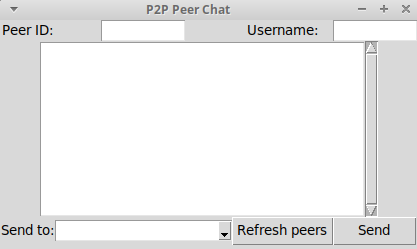
\includegraphics[width=\textwidth]{gui1}
	\caption{P2P chatovacia aplikácia}
\end{figure}

V~hornej časti obrazovky je potrebné zadať číselné ID instancie peera, ktorý je už spustený, a jeho používateľské meno (toto meno sa použije v~poli odosielateľ u~odoslanej správy). 

\begin{figure}[H]
	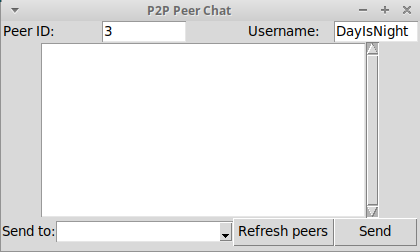
\includegraphics[width=\textwidth]{gui2}
	\caption{Údaje o~odosielateľovi}
\end{figure}

Po prvom spustení je zoznam peerov, ktorým je možné poslať správu, prázdny, a preto je potrebné tento zoznam aktualizovať pomocou tlačidla \uv{Refresh peers}.

\begin{figure}[H]
	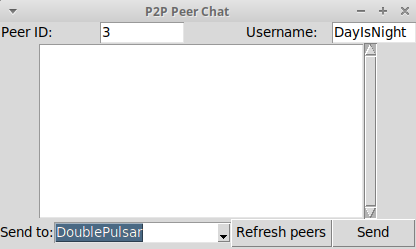
\includegraphics[width=\textwidth]{gui3}
	\caption{P2P chatovacia aplikácia}
\end{figure}

Následne si používateľ môže zoznamu peerov vybrať, komu chce správu adresovať a do textové poľa zadať obsah správy.

\begin{figure}[H]
	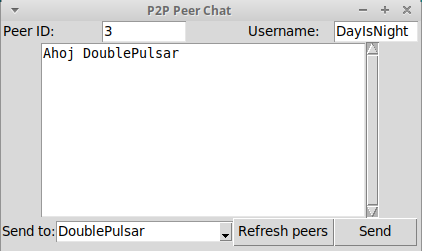
\includegraphics[width=\textwidth]{gui4}
	\caption{Obsah správy}
\end{figure}

Ak nenastal žiadny problém pri posielaní správy a správa dorazila na cieľového peera, na strane príjemcu je možné vidieť prijatú stranu.

\begin{figure}[H]
	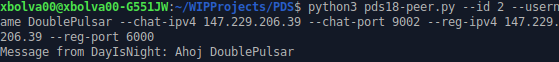
\includegraphics[width=\textwidth]{gui5}
	\caption{Prijatá správa}
\end{figure}

\chapter{Ladenie a testovanie}

Priebežné ladenie a testovanie implementácie prebiehalo na mojom notebooku so systémom s~Ubuntu 18.04 LTS a Pythonom 3.6. Takmer finálna implementácia bola následné otestovaná spolu s~implementáciami ďalších spolužiakov, kde sa opravili nájdené chyby. Na záver prebehlo záverečné testovanie implementácie aj na referenčnom virtuálnom stroji pre tento projekt.

\section{Individuálne ladenie implementácie}
Vytvorené programy som priebežne ladil prevažne pomocou ladiacich výpisov. Prebiehajúcu UDP/TCP komunikáciu som sledoval pomocou nástroja Wireshark.

\begin{figure}[H]
	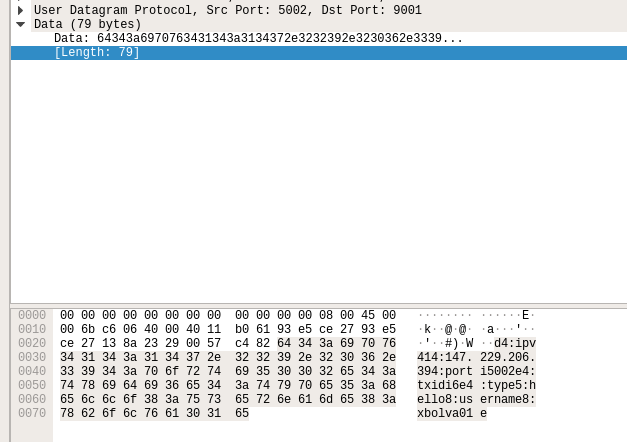
\includegraphics[height=10cm, width=\textwidth]{wireshark}
	\caption{Príklad sledovanie komunikácie vo Wiresharku \-- HELLO správa (peer $\rightarrow$ registračný uzol)}
\end{figure}

\begin{figure}[H]
	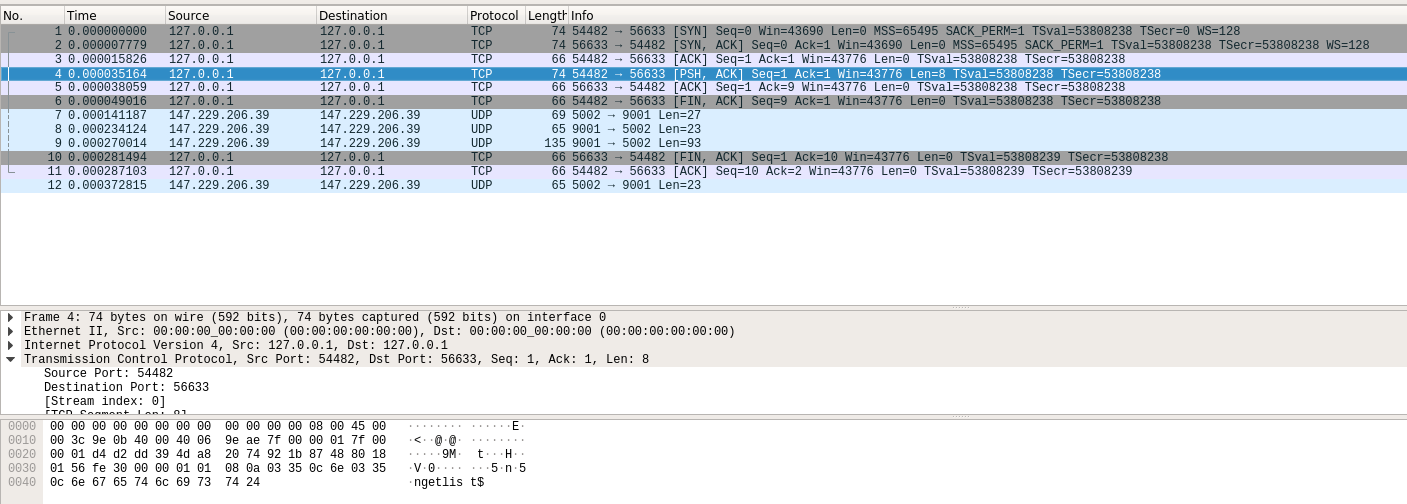
\includegraphics[width=\textwidth]{wireshark2}
	\caption{Príklad sledovania komunikácie Wiresharku \-- RPC príkaz GETLIST. V~záznamoch z~Wiresharku je možné vidieť moment poslania príkazu GETLIST peerovi cez RPC, tj. naviazalo sa TCP spojenie medzi RPC a peerom. V~záznamoch nasleduje UDP komunikácia, kde peer poslal správu GETLIST svojmu registračnému uzlu, peerovi prišiel ACK na GETLIST a aj LIST od registračného uzla. Peer následne poslal ACK registračnému uzlu na prijatý LIST.}
\end{figure}

\section{Testovanie na virtuálnom stroji}

Dokončenú implementáciu som otestoval na referenčnom virtuálnom stroji s~Ubuntu OS pre tento projekt. Okrem rôznych testovaných scenárov zmienim asi tej najhlavnejší \-- poslanie správy v~plne prepojenej sieti. Spustil som tri registračné uzly a troch peerov. Každý peer sa napojil na jeden zo spustených uzlov. Následne som prepojil prvý uzol s~druhým, a druhý s~tretím. Prvý registračný uzol sa následne vďaka správam \texttt{update} dozvedel o~treťom uzle a naviazal s~ním susedstvo. Ďalej som si vypísal databázy a susedov pre kontrolu stavu siete. Následne som otestoval najpodstatnejšiu službu hybridnej chatovacej P2P siete \-- posielanie správ. Po vytvorení plne prepojenej siete som teda poslal úspešne správu z~prvého peera na tretieho. Nasledujúce obrázky \ref{vm1} a \ref{vm2} dokumentujú priebeh tohto testovacieho scenáru v~termináli na virtuálnom stroji.


\begin{figure}[H]
	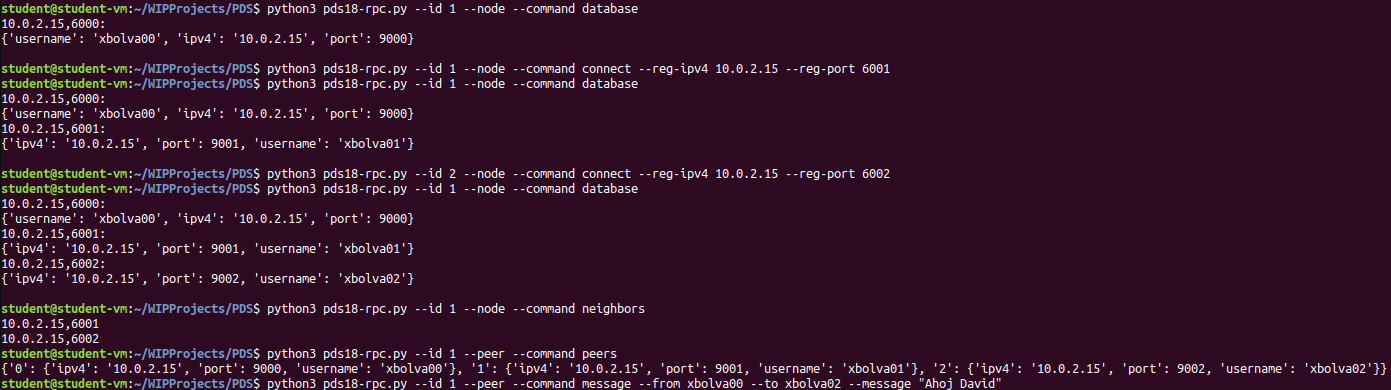
\includegraphics[width=\textwidth]{vm_fullmesh}
	\caption{Priebeh vytvorenia plne prepojenej siete a následne poslanie správy pomocou RPC}
	\label{vm1}
\end{figure}

\begin{figure}[H]
	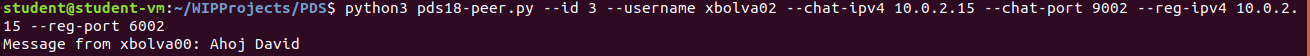
\includegraphics[width=\textwidth]{vm_prijatasprava}
	\caption{Prijatie správy  od prvého peera na strane tretieho peera}
	\label{vm2}
\end{figure}

\section{Skupinové testovanie implementácie}

Validačné a verifikačné testovanie kompatibility a funkčnosti implementácie prebiehalo spolu s~ďalšími spolužiakmi. Dňa 23. 4. 2019 som testoval projekt so 3 spolužiakmi, menovite Radimom Červinkom (xcervi21), Filipom Greplom (xgrepl05) a Lukášom Dekrétom (xdekre00). O~deň neskôr som testoval s~ďalšími spolužiakmi, a to s~Petrom Šuhajom (xsuhaj02), Lukášom Dekrétom (xdekre00), Romanom Dobiášom (xdobia11) a Petrom Rusiňákom (xrusin03). Obrázok \ref{schema} zobrazuje schému siete, z~ktorej sa odvíjali tieto dva testovania. Všetci zmienení spolužiaci, s~ktorými som testoval, mali svoje implementácie napísané v~jazyku Python. 

\begin{figure}[H]
	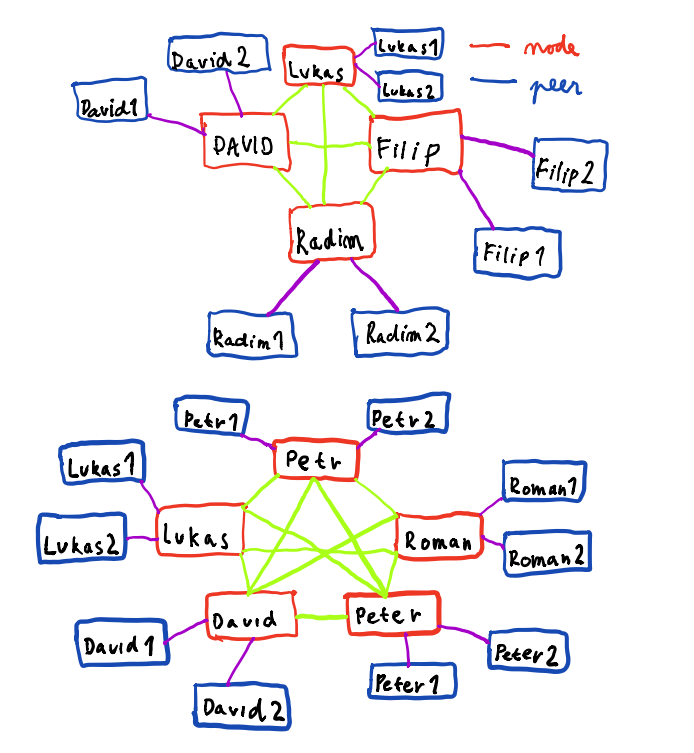
\includegraphics[width=\textwidth]{testovanie}
	\caption{Schéma siete a prepojenia registračných uzlov a peerov na začiatku testovaní}
	\label{schema}
\end{figure}


Následne v~piatok 26. 4. 2019 prebehlo tretie testovanie, kde už sa objavila aj implementácia v~jazyku C++.

\subsection{Prvé hromadné testovanie implementácie}

Pri prvom testovaní sme ja a Radim boli pripojení na Wi-Fi sieť Eduroam v~CVT na FIT VUT. Filip mal registračné uzly a peerov spustených na externom serveri. Lukáš bol pripojený ethernetom na internáte. Všetci sme si spustili registračný uzol a dvoch peerov, ktorých sme napojili na svoj registračný uzol. Následne sme prepojili naše registračné uzly, tj. vytvorili sme  full-mesh sieť a následne skúšali rôzne príkazy a scenáre. Tu sme odhalili problém Wi-Fi siete v~CVT, ktorá zabraňovala v~priamej komunikácii medzi mnou a Radimom. Komunikácia s~ďalšími spolužiakmi prebiehala úplne v~poriadku. Keďže sme skúšali aj scenáre, ktoré mali viesť k~chybovým hláseniam, pár zmien, ktoré vyplynuli z~tohto testovania sa týkalo práve obsahu hlásení na problém pri benkodódovaní, či na nesprávne správy, ktoré nespĺňajú definovaný komunikačný protokol, aby obsahovali čo najviac informácií pre druhú stranu, ktorá poslala chybnú správu. Záverom tohto prvého (skoro dvojhodinového) testovania je, že implementácie fungovali správne pri všetkých testovaných scenároch, čo nám napadli.

\subsection{Druhé hromadné testovanie implementácie}


Druhé testovanie (približne tiež dvojhodinové) prebiehalo na internátoch. Organizácia a koordinácia testovania prebieha cez skupinový hovor na Facebook Messengeri. Všetci sme si spustili registračný uzol a dvoch peerov. Najskôr sme svojich peerov napojili na svoj uzlov a následne sme skúšali rôzne príkazy a scenáre na tejto full-mesh sieti. Až na jeden prípad, keď spolužiak potvrdzoval správy nesprávnym číslom, tj. nepoužil sekvenčné číslo zo správy, na ktorú reaguje, sme nezaznamenali žiadne problémy v~implementáciách.

\subsection{Tretie hromadné testovanie implementácie}

V~piatok 26. 4. 2019 zverejnil Martin Vlnas (xvlnas00), ktorý projekt implementoval v~C++, IPv4 adresy a porty svojho registračného uzlu a peera. Svojho registračného uzla s~jedným peerom som teda napojil na jeho registračný uzol a spolu s~Petrom Rusiňákom (xrusin03), Filipom Greplom (xgrepl05) a Dominikom Polehňa (xpoleh00) \-- obaja s~Python implementáciami \-- sme vytvorili plne prepojenú sieť. Druhého peera som napojil na Petrov registračný uzol. Následne sme sa prepojil s~registračnými uzlami iných spolužiakov, ktorí ich mali pustené na merline. Vyskúšali sme všetky príkazy a posielanie správ. Fungovalo to správne. Následne sa pripojil do siete Lukáš Dekrét (xdekre00). Z~prvého peera som mu poslal správu úspešne, no z~druhého nie. Príkaz \texttt{peers} vypisoval rozdielne zoznamy aktuálnych peerov. Zistil som, že môj node posiela kompletné záznamy o~peeroch, no Petrov posielal záznamy bez informácii o~Lukášových peeroch. Zistenú chybu som mu nahlásil, aby sa na to pozrel. Okrem toho nenastali žiadne ďalšie problémy pri testovaní.

\begin{figure}[H]
	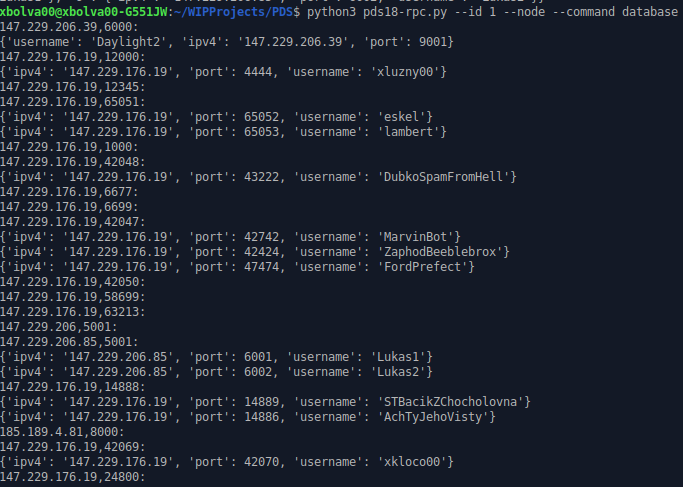
\includegraphics[width=\textwidth]{vm_fullmesh2}
	\caption{Výpis databáze pri treťom testovaní na mojom registračnom uzle}
	\label{vm1}
\end{figure}


\chapter{Použitie programov}

Projekt sa skladá s~troch programov \-- \texttt{pds18-peer}, \texttt{pds18-node} a  \texttt{pds18-rpc}.
Programy sa spúšťajú cez terminál. Pri zadaní prepínača \texttt{-h/-{}-help} sa vypíše informačný text o~programe a jeho prepínačoch. V~prípade neznámeho či chybne použitého prepínača (nesprávna/chýbajúca hodnota prepínača) alebo pri akejkoľvek chybe v~sieťovej komunikácii (napr. problém pri bindovaní, problém napojenia RPC na peera/uzol) sa program ukončí a o~probléme informuje používateľa správou na štandardný chybový výstup. Programy sa ukončujú pomocou trl-C, resp. pomocou príkazu \uv{kill -INT <pid>} v~termináli.

\section{Chatovací peer (pds18-peer)}

\begin{framed}
Použitie: pds18-peer.py [-h] --id ID --username USERNAME --chat-ipv4 CHAT\_IPV4
--chat-port CHAT\_PORT --reg-ipv4 REG\_IPV4 --reg-port
REG\_PORT\\

--id ID je číselný identifikátor instancie peera

--username USERNAME je unikátne používateľské meno identifikujúce peera v~rámci chatu

--chat-ipv4 CHAT\_IPV4 a --chat-port CHAT\_PORT je IPv4 adresa a port, na ktorom peer naslúcha a prijíma správy od ostatných peerov alebo uzlov

--reg-ipv4 REG\_IPV4 a --reg-port REG\_PORT je IPv4 adresa a port registračného uzlu, na ktorý peer bude: 1) pravidelne zasielať HELLO správy; a 2) odosielať správu GETLIST k~zisteniu aktuálneho mapovania.

-h|-{}-help zobrazenie informácii o~programe a o~prepínačoch
\end{framed}

\section{Registračný uzol (pds18-node)}

\begin{framed}
	Použitie: pds18-node.py [-h] --id ID --reg-ipv4 REG\_IPV4 --reg-port REG\_PORT\\
	
	--id ID je číselný identifikátor instancie uzla
	
	--reg-ipv4 REG\_IPV4 a --reg-port REG\_PORT je IPv4 adresa a port registračného uzlu, na ktorom prijíma registrácie uzlov a synchronizácie databázy s~ostatnými uzlami
	
	-h|-{}-help zobrazenie informácii o~programe a o~prepínačoch
\end{framed}

\section{RPC (pds18-rpc)}

\begin{framed}
	Použitie: pds18-rpc.py [-h] --id ID [--peer] [--node] --command COMMAND [COMMAND\_ARGS]
	\\
	
	--id ID je číselný identifikátor instancie uzla
	
	--peer alebo --node určuje, či sa jedná o~príkaz pre instanciu peera alebo registračného uzla
	
	--command COMMAND a zoznam parametrov COMMAND\_ARGS určujúcich príkaz a parametre vzťahujúce sa k~danému RPC príkazu
	
	-h|-{}-help zobrazenie informácii o~programe a o~prepínačoch
\end{framed}

\subsection{Príkazy RPC}

\begin{framed}
--peer --command message --from <username1> --to <username2> --message <správa>, ktorý sa pokúsi odoslať správu

--peer --command getlist, ktorý vynúti aktualizáciu zoznamu v~sieti známych peerov

--peer --command peers, který zobrazí aktuálny zoznam peerov v~sieti

--peer --command reconnect --reg-ipv4 <IP> --reg-port <port>, ktorý sa odpojí od súčasného registračného uzlu a pripojí sa k~uzlu špecifikovanému v~parametroch príkazu

--node --command database, ktorý zobrazí aktuálnu databázu peerov a ich mapovanie

--node --command neighbors, který zoznam aktuálnych susedov registračného uzla

--node --command connect --reg-ipv4 <IP> --reg-port <port>, ktorý sa pokúsi naviazať susedstvo s~novým registračným uzlom

--node --command disconnect, ktorý zruší susedstvo so všetkými uzlami a odpojí uzol od siete

--node --command sync, ktorý vynúti aktualizáciu databáze s~uzlami, s~ktorými uzol aktuálne susedí
\end{framed}

\subsection{Ukážky výpisov}
Nasledovné ukážky majú za cieľ oboznámiť používateľa RPC klienta s~obsahom a formátom odpovedí od peera / registračného uzla pri použití niektorých RPC príkazov.

\begin{itemize}
	\item Ukážkový výpis pre príkaz \texttt{python3 pds18-rpc.py --id 1 --node --command database}
	\begin{framed}
	147.229.206.39,6000:\\
	{'ipv4': '147.229.206.39', 'port': 9000, 'username': 'xbolva00'}\\
	147.229.206.39,6001:\\
	{'ipv4': '147.229.206.39', 'port': 9001, 'username': 'xbolva01'}\\
	147.229.206.39,6002:\\
	{'ipv4': '147.229.206.39', 'port': 9002, 'username': 'xbolva02'}\\
	\end{framed}

	\item Ukážkový výpis pre príkaz  \texttt{python3 pds18-rpc.py --id 1 --node --command neighbors}
	\begin{framed}
		147.229.206.39,6001\\
		147.229.206.39,6002
	\end{framed}

	\item Ukážkový výpis pre príkaz  \texttt{python3 pds18-rpc.py --id 1 --peer --command peers}
	\begin{framed}
		'0': {'ipv4': '147.229.206.39', 'port': 9000, 'username': 'xbolva00'}, \\
		'1': {'ipv4': '147.229.206.39', 'port': 9001, 'username': 'xbolva01'}, \\
		'2': {'ipv4': '147.229.206.39', 'port': 9002, 'username': 'xbolva02'}
	\end{framed}
\end{itemize}

\section{Príklady použitia}

\begin{itemize}
	\item \texttt{python3 pds18-peer.py --id 1 --chat-ipv4 147.229.206.39 --chat-port 9000\\ --username xbolva00 --reg-ipv4 147.229.206.39 --reg-port 6000}
	
	Spustí instanciu peera s~identifikátorom 1 a používateľským menom \textit{xbolva00}, ktorá sa napojí na daný registračný uzol.
	
	\item \texttt{python3 pds18-node.py --id 1 --reg-ipv4 147.229.180.26 --port 6000}
	
	Spustí instanciu registračného uzla s~identifikátorom 1, ktorý bude počúvať na danej IPv4 adrese a porte.
	
	\item \texttt{python3 pds18-rpc.py --id 1 --node --command connect --reg-ipv4 147.229.206.\\39 --reg-port 6000}
	
	Naviaže susedstvo s~registračným uzlom definovaným parametrami príkazu.
	
	\item \texttt{python3 pds18-rpc.py --id 1 --peer --command message --from xbolva00 --to Jan --message Ahoj}
	
	Pokúsi sa poslať správu \uv{Ahoj} peerovi s~používateľským menom \textit{Jan}.
\end{itemize}

\chapter{Záver}
V~rámci projektu bola naimplementovaná, otestovaná a zdokumentovaná hybridná chatovacia P2P sieť skladajúca sa z~peerov a registračných uzlov. Implementácia bola napísaná v~jazyku Python a následne bola podrobená testovaniu kompatibility a samotnej funkčnosti s~ďalšími spolužiakmi. Vďaka testovaniu sme si všetci mohli otestovať implementácie a opraviť zistené chyby a nezrovnalosti tak, aby implementácia spĺňala špecifikáciu protokolu a chovanie hybridnej chatovacej P2P siete zo zadania projektu.
